\documentclass[11 pt]{article}
\usepackage[utf8]{inputenc}
\usepackage[spanish]{babel}
\usepackage{graphicx}
\usepackage{anysize}
\marginsize{2.5cm}{2.5cm}{2.5cm}{2.5cm}
\parindent 1 cm
\usepackage{hyperref}
\hypersetup{
	colorlinks=true,
	linkcolor=black,
	urlcolor=cyan,
	citecolor=blue,
		}
\title{Situación actual de la Hepatitis E}
\author{Silvia Díaz Arco}
\date{14 de Diciembre de 2020}
\begin{document}
\maketitle
	\begin{abstract}
		Enlace al repositorio: \url{https://github.com/silviad95/Proyecto_final.git}\\\\
		La hepatitis viral es la forma más común de hepatitis. Entre los diferentes tipos posibles, la hepatitis E está emergiendo globalmente, siendo responsable de la mayoría de los casos de hepatitis aguda. El virus de la hepatitis E (VHE) es un virus de genoma ARN de cadena sencilla y polaridad positiva que pertenece al género {\em Orthohepevirus} de la familia {\em Hepeviridae}. Existen diversos genotipos, de los cuales el 1 y el 2 son patógenos humanos estrictos que se transmiten por la ruta fecal-oral debido a aguas contaminadas. Por ese motivo, son predominantes en los países en vías de desarrollo. Por otro lado, los genotipos 3 y 4 son de transmisión zoonótica, presentando una mayor variedad de huéspedes además del humano, siendo el reservorio principal el cerdo. Estos genotipos han adquirido interés al ser comunes en zonas industrializadas. La infección por VHE suele ser asintomática y autolimitante, pero precisamente por eso, en el mundo desarrollado se han dado casos de transmisión parenteral por donantes sanguíneos. Asimismo, se han documentado casos de hepatitis crónica en pacientes inmunocomprometidos. Para el diagnóstico de la infección, además de tener en cuenta el historial clínico del paciente, se recomienda la combinación de pruebas moleculares y serológicas. El tratamiento se basa en un antiviral no específico, ribavirina, no existiendo apenas terapias alternativas. Para la prevención del virus, solo existe una vacuna licenciada en China (Hecolin®), de la que no se ha probado su eficacia hacia el genotipo 3 ni su seguridad ante personas de riesgo.\\\\ 
		{\bf Palabras clave:} Hepatitis, viral, VHE, infección, genotipo	
	\end{abstract}
\tableofcontents
\newpage
\section{Introducción}
\subsection{Hablemos de Hepatitis}
El término hepatitis significa “inflamación del hígado”. Es una afección global bastante frecuente que puede remitir espontáneamente, pero, que, en algunos casos, lleva al daño y destrucción de hepatocitos. Se pueden diferenciar entre hepatitis aguda (a corto plazo) y crónica (cuando la infección se prolonga a largo plazo). Las infecciones crónicas, sobre todo cuando se diagnostican tarde y no hay tratamiento, pueden generar daño permanente en el hígado pasando por la fibrosis (cicatrices), sangrado gastrointestinal, cirrosis (cicatrices permanentes), fallo en el hígado fulminante y/o un carcinoma hepatocelular que puede llevar al paciente a la muerte \cite{Mehta2020}.\\\\
Aunque la hepatitis se deba principalmente a infecciones virales, de las que hablaremos en el siguiente párrafo, también puede darse por causas no infecciosas. Así, la inflamación del hígado puede originarse por una enfermedad autoinmune \cite{Liberal2013}, por hígado graso \cite{NeuschwanderTetri2017} o por consumo excesivo de alcohol (hepatitis alcohólica) \cite{Chayanupatkul2014} y/o medicamentos \cite{Alempijevic2017}.\\\\
Existen 5 tipos principales de hepatitis virales, que se nombran de la A a la E. Aparte, se ha descrito la existencia de la hepatitis G. Normalmente se manifiesta como una coinfección con hepatitis B y C, aunque se desconoce su importancia en humanos. Otros virus, que generalmente no afectan principalmente al hígado, pero pueden causar hepatitis, son los citomegalovirus (CMV), el virus de Epstein-Barr (EBV) o el virus del herpes simple \cite{Mehta2020}. Las características que definen a cada tipo de hepatitis se muestra en la Tabla 1.
\begin{table}[h!]
\begin{tabular}[c]{|c|c|c|c|c|c|c|}
	\hline
    	& {\bf VHA} & {\bf VHB} & {\bf VHC} & {\bf VHD} & {\bf VHE} \\
	\hline
	{\bf Género} & {\em Hepatovirus} & {\em Orthohepadnavirus}&{\em Hepacivirus}&{\em Virusoide}&{\em Orthohepevirus} \\
	\hline
	{\bf Genoma} & ARNss+ & ARNds parcial & ARNss+ & ARN & ARNss+\\
	\hline
	\parbox[c]{2 cm}{{\bf Fuente principal de transmisión}}
 & Ruta fecal-oral & \parbox[c]{2 cm}{Vertical, parenteral, sexual} & \parbox[c]{2 cm}{Contacto sanguíneo} & \parbox[c]{2 cm}{Coinfección o superinfección con VHB, contacto por sangre} & \parbox[c]{2 cm}{Ruta fecal-oral (países en desarrollo) Zoonótica (países desarrollados)}\\
	\hline 
	\parbox[c]{1.75 cm}{{\bf Tipo de infección}} & Aguda & Aguda y crónica & Crónica & \parbox[c]{2 cm}{Agrava pronóstico VHB} & Aguda y crónica\\
	\hline
	{\bf Tratamiento} & No específico & Sí (crónico) & Sí & Igual VHB & Sí (crónico)\\
	\hline
	{\bf Prevención} & Vacuna & Vacuna & Cribado & Igual VHB & \parbox[c]{2 cm}{Vacuna (solo en China)}\\
	\hline
\end{tabular}
\end{table}
\footnote[1]{{\bf Tabla 1}. Características de cada hepatitis. Significado de las siglas y referencias: VHA virus de la hepatitis A \cite{Thuener2017}, VHB virus de la hepatitis B \cite{You2014}, VHC virus de la hepatitis C \cite{Li2015}, VHD virus de la hepatitis D \cite{Rizzetto2015} y VHE virus de la hepatitis E \cite{Mohsen2017}. }

\subsection{Incidencia global}
En la figura \ref{laninigrafico} se muestra un gráfico circular que representa los datos de muertes por las diferentes hepatitis virales en 2017. Se puede observar que los pacientes mayores de 50 años son los que tienen más riesgo, ya que la tasa de mortalidad se dispara hacia 1.300.000. Asimismo, se puede ver que la principal causa de esas muertes es por la evolución crónica de la hepatitis B y C. En los individuos jóvenes, sin embargo, el fallo hepático agudo es el principal origen de esas muertes (89\%). Hay que destacar, además, que la hepatitis E fue causante de unos 1.500 fallecimientos en personas jóvenes y de unas 13.250 muertes en personas mayores de 50 años \cite{Lanini2019}.
\begin{figure} [h!] 
	\centering
	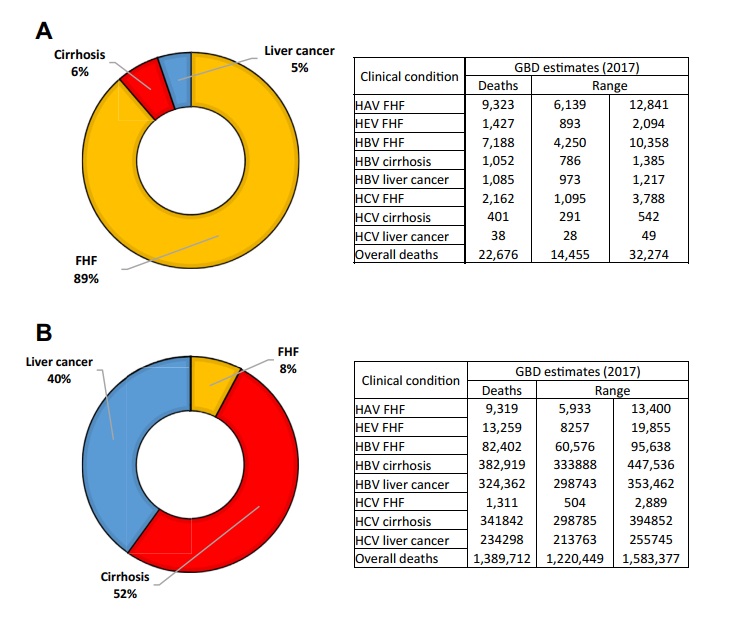
\includegraphics[width=0.75\linewidth]{imagenes/graficoincidenciahepatitis.png}
	\caption[loftitle]{Representación de muertes asociadas con las diferentes hepatitis virales en gente de menos de 50 años (A) y mayores de 50 años (B). Tomado de Lanini et al (2019) \cite{Lanini2019}}
	\label{laninigrafico}
\end{figure}

Actualmente, se reconoce el interés sanitario de la hepatitis E tanto en los países en desarrollo como en los países industrializados, donde se han dado casos de progresión de la hepatitis hacia una evolución crónica. Además, es una enfermedad emergente que es causante de la mayoría de casos de hepatitis aguda globalmente. Partiendo del creciente interés que ha suscitado esta infección, se ha querido realizar una búsqueda bibliográfica para recoger la información actualizada y completa que existe sobre esta patología. Con ello, también se pretende destacar dónde es necesario continuar investigando.

\section{Materiales y métodos}
\subsection{Tipo de estudio}
Para la comprobación del estado del arte se ha elegido, en primer lugar, llevar a cabo una revisión bibliográfica. Para ello, se ha realizado una búsqueda en diferentes de datos utilizando varias combinaciones y operadores booleanos. Se hizo una selección de los artículos científicos más actualizados y una lectura exhaustiva y crítica de cada uno de ellos, realizando siempre una valoración de la información disponible. 
\subsection{Búsqueda bibliográfica}
Las bases de datos elegidas para la realización de la búsqueda de bibliografía fueron Pubmed, Web of Science y Scopus.\\\\  
Se realizó una búsqueda sobre la hepatitis E mediante las palabras clave “Hepatitis E”, “Orthohepevirus”, “VHE” and “diagnosis”, “Hepatitis E” and “clinical manifestation” y “Hepatitis E” and “treatment”. \\\\\
Para acotar la búsqueda se fijaron varios criterios de selección y rechazo. Se utilizó el filtro “review” para que se mostraran preferentemente las revisiones bibliográficas. Además, en el caso de que el número de artículos siguiese siendo alto, se limitaba también el tiempo de publicación para que fuesen todos recientes (5 años). Además de la fecha de publicación, también se tenía en cuenta el mayor número de citaciones de los artículos y el buen índice de impacto de las revistas en las que se han publicado, eligiéndose preferentemente estos artículos de otras revisiones sobre el mismo tema. En el caso de artículos donde se prueban diferentes métodos de diagnóstico, se ha tenido en cuenta que el estudio fuese íntegramente en humanos, que se analicen un número alto de muestras con los criterios de calidad pertinentes y con resultados válidos, indicando siempre la sensibilidad y especificidad del método. El idioma elegido, además, podría ser inglés o español.\\\\ 
Por otro lado, se han rechazado los artículos de otras enfermedades que no fuesen hepatitis E, o que tratasen de esta patología en animales. También se han descartado artículos con más de 5 años de antigüedad.\\\\    
Atendiendo a estos criterios, al final se han seleccionado tres artículos para realizar el estado del arte. 

\section{Conclusiones}
Tras la búsqueda de los artículos más relevantes y actualizados de la patología de la Hepatitis E, se puede destacar los siguientes puntos:
\begin{itemize}
	\item 
	La infección por VHE ha dejado de considerarse anecdótica y asociada a viajero en países desarrollados, siendo los genotipos 3 y 4 los más frecuentes en estos países. La transmisión de estos genotipos es zoonótica, siendo el ganado porcino el principal reservorio. 
	\item 
	Los genotipos 3 y 4 pueden producir hepatitis crónica en personas inmunocomprometidas, principalmente trasplantados.
	\item 
	Existe relación de infección por genotipos 3 y 4 y manifestaciones extrahepáticas (neurológicas, renales y hematológicas), aunque la relación causa efecto aún está en estudio.
	\item 
	Existe controversia respecto a la necesidad de cribado del VHE en donantes de sangre y órganos.
	\item 
	Falta por establecer dosis y tiempo del tratamiento con ribavirina
	\item 
	Existen muchos ensayos para diagnóstico serológicos, aunque ninguno ha sido aún aprobado por la FDA. Falta estandarización en estos ensayos
	\item 
	En cuanto a la prevención, se basa en medidas higiénico sanitarias en países en vías de desarrollo y evitar consumo de carnes poco cocinadas. Solo existe una vacuna licenciada en China, denominada Hecolin® {\em (Xiamen Innovax Biotech)}. La OMS no la ha integrado en programas de vacunación globales porque se necesita probar su eficacia con respecto a otros genotipos y su seguridad en pacientes de riesgo.
\end{itemize}
Por consiguiente, es necesario continuar los esfuerzos de investigación en los puntos destacados donde hay desconocimiento. Al final, el objetivo es poder realizar un buen tratamiento y, sobre todo, crear una vacuna global para lograr una prevención eficaz.



\bibliography{biblio_proyectofinal}
\bibliographystyle{unsrt}		
\end{document}